\documentclass[aspectratio=169]{beamer}

\usepackage[utf8]{inputenc}

\usepackage{standalone}
\usepackage{caption}
\usepackage{amssymb, amsmath, amsthm, amsfonts}

\usepackage{tikz}
\usepackage{pgfplots}
\usetikzlibrary{shapes.geometric, arrows}
\usetikzlibrary{backgrounds}
\tikzstyle{node} = [rectangle]

\usepackage{float}

\newcommand{\comment}[1]{}

\usetheme{Dresden}
\usepackage[orientation=landscape,size=custom,width=16,height=9,scale=0.5,debug]{beamerposter}
\usepackage{animate}
\usepackage{url}

\title{N-body memory layout exploration}
\author{Oliver Geisel \& Lisa Hentschke}
\date{\today}


\begin{document}

\begin{frame}
	\titlepage
\end{frame}

\begin{frame}
	\frametitle{Structure}
	\tableofcontents
\end{frame}

\section{The task} 
\begin{frame}
	\frametitle{The n-body simulation}
	\begin{columns}
	\begin{column}{0.55\textwidth}
		\begin{itemize}
			\item simulate the interaction of \(n\) particles
			\item each particle has
			\begin{itemize}
				\smallskip
				\item position x
				\item position y
				\item position z
				\smallskip
				\item velocity x
				\item velocity y
				\item velocity z
				\smallskip
				\item mass
			\end{itemize}
		\end{itemize}
	\end{column}
	
	\begin{column}{0.45\textwidth}
		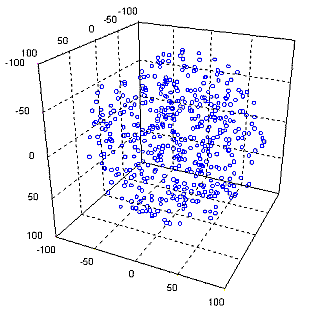
\includegraphics[scale=0.65]{resources/nbody.png}
		\tiny \url{http://astro.dur.ac.uk/~nm/pubhtml/nbody/nbody.html}
	\end{column}
	
	\end{columns}
	
\end{frame}

\section{Results} 
\begin{frame}
	\frametitle{Compare the memory structures}
	
\end{frame}

\end{document}